\chapter{Research Results and Discussion}\label{chap:research_results}

This chapter presents the experimental results in five sections that build directly on one another. Section~\ref{sec:res_data} characterises the collected sensor data across all five experimental batches. Section~\ref{sec:res_energy} profiles the energy consumption of every hardware component in the sensing node, answering SQ1. Section~\ref{sec:res_ml} compares the four ML framework configurations in energy and accuracy, answering SQ2 and SQ3. Section~\ref{sec:res_battery} translates the measured energy profiles into estimated battery lifetime across three hardware scenarios, answering SQ4. Section~\ref{sec:res_discussion} synthesises all four answers, provides deployment recommendations, and discusses limitations and broader impact.

All energy measurements were obtained using a Nordic Semiconductor PPK2 operating at \SI{3.3}{\volt}, repeated across three independent runs; values are reported as mean $\pm$ standard deviation. Accuracy metrics were evaluated on the held-out Batch~5 test set (332 samples: 110 mould-positive, 222 mould-negative) that was not used at any point during training or validation.

% ─────────────────────────────────────────────────────────────────────────────
\section{Collected Environmental Data}\label{sec:res_data}
% ─────────────────────────────────────────────────────────────────────────────

\subsection{Dataset Overview}\label{subsec:res_dataset_overview}

Five experimental batches of strawberry samples were collected over the course of this project, yielding 1,653 readings across the three-node sensing system. Figure~\ref{fig:data_overview} summarises the per-batch composition: the left panel shows how many readings in each batch fall before and after the confirmed mould-onset point, and the right panel shows how many readings were flagged as TVOC-saturated.

\begin{figure}[htbp]
    \centering
    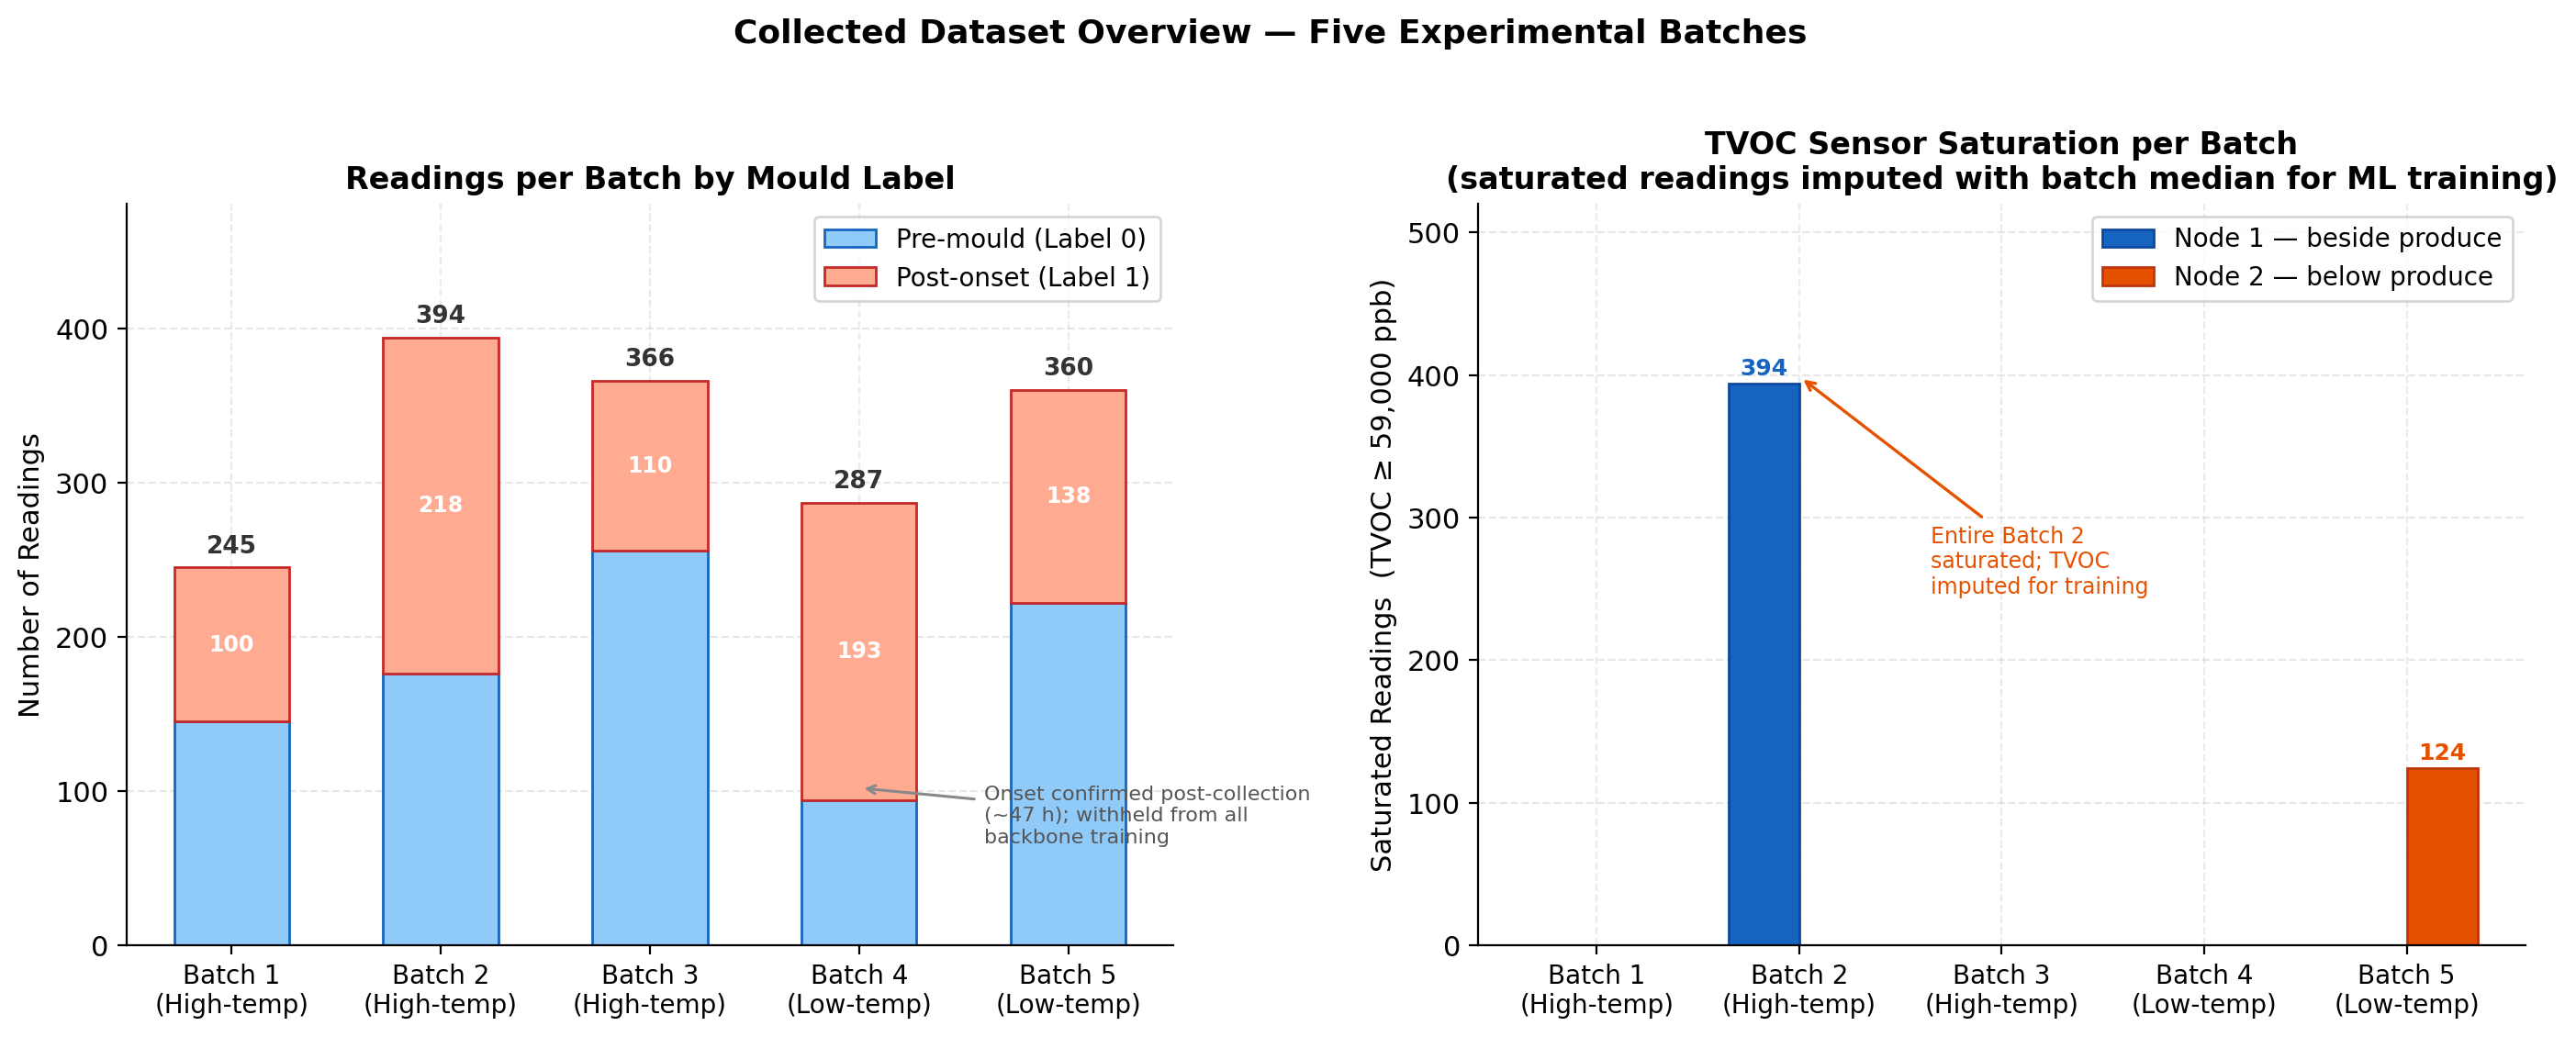
\includegraphics[width=\textwidth]{images/fig_data_overview.png}
    \caption{Left: readings per batch divided into pre-mould (Label~0) and post-onset (Label~1) samples. Batch~4 was withheld from backbone training and used for TinyOL on-device fine-tuning; it was also included in the AIfES full on-device training corpus. Right: TVOC saturation counts per batch (SGP30 ceiling \SI{59000}{ppb}). Saturated readings are imputed with the per-batch median TVOC before training; rows are not discarded.}
    \label{fig:data_overview}
\end{figure}

Table~\ref{tab:batch_summary} summarises each batch's experimental regime, data quality, and role in the ML pipeline.

\begin{table}[H]
\centering
\caption{Summary of experimental batches --- regime, data quality, and ML pipeline role.}
\label{tab:batch_summary}
\begin{tabular}{|c|p{0.10\textwidth}|c|p{0.36\textwidth}|p{0.22\textwidth}|}
\hline
\textbf{Batch} & \textbf{Regime} & \textbf{Onset} & \textbf{Primary data quality note} & \textbf{ML role} \\
\hline
1 & High-temp & $\approx$36\,h & Node~1 entered with elevated TVOC ($\approx$39,700\,ppb); close to sensor ceiling & Backbone fit set \\
\hline
2 & High-temp & $\approx$44\,h & All inside-node TVOC saturated throughout; TVOC imputed with batch median & Backbone fit set (imputed TVOC); TinyOL val set \\
\hline
3 & High-temp & $\approx$64\,h & Cleanest batch; temp SD \SI{0.55}{\celsius}, unambiguous onset progression & Backbone early-stopping validation \\
\hline
4 & Low-temp & $\approx$47\,h & Onset timestamp confirmed post-collection; low-temperature regime & TinyOL fine-tuning; AIfES full training corpus \\
\hline
5 & Low-temp & $\approx$55\,h & Node~2 near-saturated pre-onset, compressing post-onset dynamic range & Held-out test set \\
\hline
\end{tabular}
\end{table}

The backbone model used for AIfES inference and TF Lite Micro was fit on Batches~1 and~2 (gradient updates), with Batch~3 used exclusively for early-stopping validation. Batch~4 was withheld from backbone training and served two roles: it provided the fine-tuning dataset for TinyOL on-device output-layer adaptation, and it was included in the AIfES full on-device training corpus alongside Batches~1--3. Batch~5 was held out as the final test set and was never used in any form of training or validation.

\subsection{Sensor Time Series — Batch~3 Representative}\label{subsec:res_timeseries}

Figure~\ref{fig:sensor_trends} shows the complete Batch~3 time series across all four sensing channels. Batch~3 is selected as the representative example because it offers the cleanest progression across every channel: temperature was controlled to within \SI{0.55}{\celsius} standard deviation, the TVOC baseline was well below the saturation ceiling before onset, and the mould-onset transition is unambiguous.

\begin{figure}[htbp]
    \centering
    \includegraphics[width=\textwidth]{images/fig_sensor_trends.png}
    \caption{Batch~3 sensor readings over time for Node~1 (beside produce, blue), Node~2 (below produce, orange), and the master node (ambient outside, grey). The dashed red line marks the recorded mould-onset point at approximately 64~hours. TVOC is zoomed to the actual signal range to clearly show the post-onset rise. Note the stronger ethanol response at Node~2 compared to Node~1 post-onset, consistent with molecular weight stratification of heavier alcohol compounds near the base of the container.}
    \label{fig:sensor_trends}
\end{figure}

Several key patterns emerge. Temperature cycles predictably in response to the heating controller: there is no step-change at the mould-onset boundary, confirming that temperature variations are artefacts of the experimental control system rather than mould-driven changes. Humidity varies smoothly and similarly does not indicate mould onset in isolation.

TVOC is the most diagnostically informative channel. Following mould onset, both inside nodes show a sustained, monotonic increase in VOC concentration while the master node outside the container remains flat. This spatial contrast confirms that the rising signal originates from the strawberry environment rather than laboratory ambient air. Node~2, positioned below the produce, rises more steeply than Node~1 beside it: dense VOC biomarkers of \textit{Botrytis cinerea} --- including 1-octen-3-ol and short-chain alcohols --- accumulate near the base of the enclosed space where Node~2 is placed.

Ethanol (MQ3) provides an interesting spatial signature. Node~2, positioned below the produce, registers substantially higher ethanol concentrations post-onset than Node~1 beside it. This is consistent with the known molecular weight stratification of gas-phase ethanol (\SI{46}{\gram\per\mole}) and heavier \textit{Botrytis cinerea} metabolites: denser molecules accumulate near the base of the enclosed container, where Node~2 is mounted. This vertical stratification effect --- lighter VOCs detected first at sensor height, heavier alcohols concentrated near the floor --- is corroborated by the literature on gas stratification in enclosed post-harvest storage environments and provides a physical interpretation for Node~2's consistently stronger ethanol signal.

\subsection{Cross-Batch Onset Consistency}\label{subsec:res_onset}

While Batch~3 offers the cleanest individual time series, it is important to verify that the VOC onset signal is consistent across all batches and not specific to one set of experimental conditions. Figure~\ref{fig:onset_alignment} addresses this directly by aligning all five batches to their recorded mould-onset point using Node~1. Node~1 is used for this comparison because Node~2 exhibits more saturation across batches; Node~1 provides cleaner cross-batch traces.

\begin{figure}[htbp]
    \centering
    \includegraphics[width=\textwidth]{images/fig_onset_alignment.png}
    \caption{TVOC readings from Node~1 (beside produce) aligned to the mould-onset event for all five batches. Left panel: TVOC traces normalised to each batch's own pre-onset baseline; all batches converge to 1.0 at $t = 0$ and rise post-onset. Right panel: raw TVOC values (ppb). Batch~2 (grey dotted) is shown but saturated throughout; its TVOC was imputed with the batch median for training. Batch~4 (purple) uses the onset timestamp confirmed post-collection.}
    \label{fig:onset_alignment}
\end{figure}

The normalised traces reveal a consistent structural pattern across all five batches: TVOC at Node~1 rises monotonically following mould onset, regardless of the absolute pre-onset level. This relative rise is reproducible across both the high-temperature (Batches~1--3) and low-temperature (Batches~4--5) experimental regimes. Batch~2's saturation is clearly visible as a plateau immediately at the onset point; its TVOC values were imputed with the batch median for training.

The normalised view is considerably more informative than the raw trace, which is also shown in the right panel for completeness. In the raw panel, Batch~1's pre-existing elevated baseline (approximately \SI{39700}{ppb} at Node~1 before any mould onset) pushes the y-axis high enough that the lower-baseline batches appear compressed near the bottom. Batch~2's saturation ceiling distorts the scale further. Normalisation removes these absolute differences and makes the shape of the post-onset rise directly comparable across all batches, which is what matters for classifier generalisation.

Excluding Batch~1 (which entered with a pre-existing elevated baseline) and Batch~2 (saturated throughout), the Node~1 TVOC value at the moment of recorded mould onset was \SI{6864}{ppb} for Batch~3, \SI{5686}{ppb} for Batch~4, and \SI{9164}{ppb} for Batch~5. These three values cluster in the range of approximately 5,700--9,200\,ppb --- a remarkably consistent band given that Batches~3 and~4--5 were conducted at different temperature regimes. This clustering suggests a biologically meaningful VOC detection threshold: \textit{Botrytis cinerea} activity becomes detectable by the SGP30 when accumulated TVOC reaches roughly \SI{6000}{}--\SI{9000}{ppb} at Node~1, regardless of temperature condition. This observation implies that a simple threshold-based alert (raise an alarm when TVOC exceeds $\approx$\SI{6000}{ppb} from a clean baseline) could act as a lightweight pre-classifier even before any ML inference is needed.

The implication for machine learning is important: models trained on one set of absolute VOC levels may encounter different baselines in new deployments, but the post-onset trajectory --- a sustained increase relative to the pre-onset stable state --- is a stable, cross-batch indicator of \textit{Botrytis cinerea} activity. This is precisely the pattern that the trained classifier must learn to detect.

% ─────────────────────────────────────────────────────────────────────────────
\section{Node Energy Consumption}\label{sec:res_energy}
% ─────────────────────────────────────────────────────────────────────────────

\subsection{Component-Level Power Breakdown}\label{subsec:res_power_breakdown}

PPK2 measurements of the slave-node hardware reveal that the average per-cycle current is dominated almost entirely by passive sensor loads rather than the microcontroller. Table~\ref{tab:power_breakdown} lists the measured or manufacturer-specified current for each component in the current hardware configuration.

\begin{table}[H]
\centering
\caption{Slave-node current breakdown --- current hardware configuration. All values are average current per 15-minute sensing cycle at \SI{3.3}{\volt}. MQ3 current was measured separately via PPK2 since it was externally powered during testing; all other values include that sensor in the PPK2-measured node current.}
\label{tab:power_breakdown}
\begin{tabular}{|p{0.24\textwidth}|c|c|p{0.46\textwidth}|}
\hline
\textbf{Component} & \textbf{Current} & \textbf{Share} & \textbf{Notes} \\
\hline
MQ3 ethanol sensor (heater) & \SI{103.3}{\milli\ampere} & 61.5\% & All three MQ3 heaters measured together at 310\,mA via PPK2; 103.3\,mA per node at 3.3\,V \\
\hline
SGP30 VOC sensor & \SI{48.0}{\milli\ampere} & 28.6\% & Continuous; no gating circuit in current hardware \\
\hline
DevKit board (LDO + USB-UART) & \SI{10.0}{\milli\ampere} & 5.9\% & Fixed overhead of development board regulators \\
\hline
ESP32 + DHT22 (duty-cycle avg) & \SI{6.75}{\milli\ampere} & 4.0\% & Includes deep-sleep and active-window average \\
\hline
\textbf{Total} & \textbf{\SI{168.1}{\milli\ampere}} & \textbf{100\%} & Per slave node; master measured at \SI{88.8}{\milli\ampere} (excl.\ MQ3); total three-node mesh $\approx$\SI{528}{\milli\ampere} \\
\hline
\end{tabular}
\end{table}

The wireless transmission step (ESP-NOW) takes approximately \SI{3}{\milli\second} per cycle and consumes less than \SI{2}{\milli\joule} per cycle --- under 0.01\% of the daily energy budget and operationally negligible.

The ESP32 chip itself achieves approximately \SI{10}{\micro\ampere} in deep sleep. The \SI{6.75}{\milli\ampere} figure in Table~\ref{tab:power_breakdown} is the duty-cycle average over the full 900-second sensing cycle, which includes brief active-phase windows for SGP30 warm-up, sensor readings, ML inference, and ESP-NOW packet transmission.

The SGP30 requires a 45-second warm-up at power-on before its metal oxide sensing element reaches thermal equilibrium and produces reliable TVOC readings. Because the SGP30 cannot be power-gated without additional circuitry in the current devkit hardware, it draws its full \SI{48}{\milli\ampere} continuously --- including throughout the deep-sleep window when no measurements are taken. This continuous draw makes the SGP30 the second-largest energy consumer despite its warm-up being only 5\% of the 15-minute cycle.

The MQ3's resistive heater is the dominant load at \SI{103.3}{\milli\ampere} per node, accounting for 61.5\% of average current. Its thermal stabilisation time exceeds the 15-minute sensing interval, making duty-cycling impractical without fundamentally changing the measurement protocol.

Figure~\ref{fig:power_breakdown} illustrates the current-node breakdown alongside an improved configuration in which the MQ3 is replaced by a low-power MEMS gas sensor and the SGP30 is power-gated with a MOSFET between readings.

\begin{figure}[htbp]
    \centering
    \includegraphics[width=\textwidth]{images/fig_power_breakdown.png}
    \caption{Average per-cycle current breakdown for the slave node. Left: current hardware with the MQ3 heater dominant, total \SI{168.1}{\milli\ampere}. Right: improved hardware with MEMS sensor replacing MQ3 and SGP30 duty-gated at 5\% on-time, total \SI{19.33}{\milli\ampere} --- an 88.5\% reduction. The DevKit board overhead (10\,mA) and ESP32 (6.75\,mA) remain unchanged in this scenario; they become the dominant consumers in the improved design, motivating a custom PCB as a further improvement.}
    \label{fig:power_breakdown}
\end{figure}

Two targeted hardware changes account for the 88.5\% reduction in average per-slave current:

\begin{enumerate}
    \item \textbf{MQ3 to MEMS replacement.} A low-power MEMS gas sensor (\SI{3.6}{\milli\ampere} active, microamp-level standby) replaces the MQ3 heater. Duty-cycled at 5\% (45-second on-time per 15-minute cycle), the effective average draw drops to \SI{0.18}{\milli\ampere} --- removing 61.3\% of total node current in a single hardware change. It is worth noting that MOSFET gating of the MQ3 itself is theoretically possible but impractical: the MQ3 heater requires many hours of thermal stabilisation before producing stable, reliable readings, making short duty cycles unsuitable for accurate ethanol measurement.
    \item \textbf{SGP30 MOSFET gate.} A low-side MOSFET controlled by a GPIO pin switches the SGP30 off between readings, limiting power-on time to the 45-second warm-up each cycle. This reduces the SGP30's effective average draw from \SI{48}{\milli\ampere} to \SI{2.40}{\milli\ampere}, addressing the second-largest energy consumer.
\end{enumerate}

After these two changes, the \SI{10}{\milli\ampere} DevKit board overhead --- fixed by the development board's on-board LDO regulator and USB-UART bridge --- becomes the largest single consumer at 51.7\% of the improved total. This motivates a natural next step: replacing the DevKit with a custom PCB and an efficient LDO regulator (e.g.\ MCP1700 with \SI{1.6}{\micro\ampere} quiescent current) could reduce board overhead to approximately \SI{1}{\milli\ampere}, bringing per-slave node current to approximately \SI{7.93}{\milli\ampere} and enabling the multi-week autonomous deployment explored in Section~\ref{sec:res_battery}.

\subsection{Effect of ESP32 CPU Frequency on Node Current}\label{subsec:res_cpu_freq}

The ESP32 supports three common operating frequencies: 240\,MHz, 160\,MHz, and 80\,MHz. Reducing frequency is a standard technique for MCU energy reduction, and it was measured here to determine whether it offers meaningful savings in this sensing application.

These measurements were taken with the MQ3 externally powered and excluded from the PPK2 circuit, isolating the SGP30, DevKit, ESP32, and DHT22 components. This is consistent with the methodology used for all other PPK2 energy measurements in this thesis.

PPK2 measurements of the slave nodes at all three frequencies showed negligible variation. At 240\,MHz, Node~1 averaged \SI{64.75}{\milli\ampere} and Node~2 averaged \SI{66.14}{\milli\ampere}. Dropping to 160\,MHz produced figures of \SI{65.58}{\milli\ampere} and \SI{66.81}{\milli\ampere} --- a marginal difference of under \SI{1}{\milli\ampere}. At 80\,MHz, Node~1 measured approximately \SI{65.1}{\milli\ampere}. The master node followed the same pattern, averaging \SI{88.79}{\milli\ampere} at 240\,MHz versus \SI{90.94}{\milli\ampere} at 160\,MHz.

Notably, the measured current is slightly \textit{higher} at lower frequencies rather than lower. This is counterintuitive from a power-consumption perspective, but the explanation is straightforward: at a lower clock speed, the ESP32 takes longer to complete each active-phase computation (SGP30 warm-up, sensor reads, inference, ESP-NOW transmission). The active window therefore occupies a larger fraction of the 15-minute cycle. Although the instantaneous active-state current is somewhat lower at reduced frequency, the longer active window more than offsets this, and the continuous \SI{48}{\milli\ampere} SGP30 draw remains constant regardless. The net average current across the full cycle is therefore marginally higher at lower clock speeds. The effect is small (under 1\,mA) because the SGP30 dominates the budget and makes both the active and sleep windows similar in current draw.

The practical conclusion is that 240\,MHz should be retained. Reducing clock speed provides no energy benefit in this sensor configuration, and running at full speed maximises ML inference performance and minimises the active window duration. If MCU frequency reduction is to be revisited, the prerequisite is first MOSFET-gating the SGP30, which would make the ratio of active-window MCU current to total node current large enough for frequency to matter.

% ─────────────────────────────────────────────────────────────────────────────
\section{Machine Learning Framework Comparison}\label{sec:res_ml}
% ─────────────────────────────────────────────────────────────────────────────

Four ML configurations were evaluated: AIfES inference (float32, frozen model weights deployed from offline training), TF Lite Micro inference (INT8 post-training quantised), TinyOL output-layer adaptation (17 trainable parameters, float32 backbone frozen), and AIfES full on-device training (all 193 parameters trained on the device, 20 epochs with Adam optimiser). All configurations were tested on the same held-out Batch~5 test set. Table~\ref{tab:ml_summary} gives the key measurements for each configuration.

\begin{table}[H]
\centering
\caption{ML framework measurements --- ESP32 @ 240\,MHz (mean $\pm$ SD, 3 PPK2 runs). Peak RAM includes all framework heap allocations. AIfES Full BSS includes 57.4\,KB shuffle buffers for on-device training.}
\label{tab:ml_summary}
\begin{tabulary}{\textwidth}{|L|c|c|c|c|c|}
\hline
\textbf{Configuration} & \textbf{ML energy} & \textbf{Latency} & \textbf{On-device} & \textbf{Peak RAM} & \textbf{Accuracy} \\
 & \textbf{per op.} & \textbf{per op.} & \textbf{params} & \textbf{(KB)} & \textbf{(\%)} \\
\hline
AIfES inference (float32)           & $6305 \pm 161$\,nJ    & \SI{45.7}{\micro\second}   & 0   & 30.1        & 94.0 \\
\hline
TF Lite Micro (INT8)                & $8881 \pm 466$\,nJ    & \SI{73.2}{\micro\second}   & 0   & 30.2        & 93.7 \\
\hline
TinyOL update (17 params)           & $1810 \pm 198$\,nJ    & \SI{13.1}{\micro\second}   & 17  & 31.2        & 86.1 \\
\hline
AIfES full training (193 params)    & $194816 \pm 13888$\,nJ & \SI{1.91}{\milli\second}  & 193 & 90.7        & 77.1 \\
\hline
\end{tabulary}
\end{table}

\subsection{Energy and Latency}\label{subsec:res_energy_latency}

Figure~\ref{fig:ml_comparison} presents the four-way comparison on log-scale axes for energy and latency, alongside horizontal accuracy bars. Log scale is necessary because the energy range spans more than two orders of magnitude: from TinyOL at \SI{1.81}{\micro\joule} per update to AIfES full training at \SI{194.8}{\micro\joule} per step.

\begin{figure}[htbp]
    \centering
    \includegraphics[width=\textwidth]{images/fig_ml_comparison.png}
    \caption{Three-panel ML framework comparison. Left and centre use log scales to display all four configurations together given the 107$\times$ energy range. Right: prediction accuracy on the 332-sample held-out Batch~5 test set; the dashed line at 90\% marks a reference threshold for high-reliability deployment.}
    \label{fig:ml_comparison}
\end{figure}

AIfES inference consumed 29\% less energy than TF Lite Micro and completed the forward pass in 37\% less time, despite using unquantised float32 arithmetic. Two factors explain this counterintuitive result. First, the network is small (193 parameters), so the TFLM runtime's flat buffers and interpreter metadata (2548-byte model file versus AIfES's 772-byte weight array) impose a larger relative overhead than the INT8 quantisation saving provides. Second, the ESP32's Xtensa LX6 processor includes a hardware floating-point unit (FPU) for single-precision arithmetic; AIfES's float32 matrix operations run natively on this FPU, while TFLM's INT8 operations go through software integer kernels that do not benefit from the FPU. At this network scale, the FPU advantage outweighs the memory-bandwidth saving of 8-bit quantisation.

TinyOL's output-layer update is the most energy-efficient single operation at \SI{1.81}{\micro\joule}, requiring only 3,146 CPU cycles for a combined forward--backward pass through the 17 output-layer parameters. Its low cost reflects the frozen backbone: feature extraction layers are not updated, so no gradient flows through the bulk of the network.

AIfES full training consumes 107$\times$ more energy per gradient step than a TinyOL update and takes \SI{1.91}{\milli\second} per step --- still short in absolute terms, but 144$\times$ longer than a TinyOL update. The high standard deviation in AIfES full training energy ($\pm$13,888\,nJ, 7.1\%) reflects variability in Adam optimiser accumulator terms across later training epochs as weight updates become smaller.

\subsection{Prediction Accuracy}\label{subsec:res_accuracy}

All accuracy figures were evaluated on the held-out Batch~5 test set of 332 samples (241 mould-positive, 91 mould-negative), which was never used in any training or validation step. With a test set of this size, a one-percentage-point difference corresponds to approximately three or four samples, so reported accuracy values carry non-negligible sampling variance. The ordering of configurations and the magnitude of the gaps are the more reliable findings; the exact percentages should be treated as estimates.

AIfES inference and TF Lite Micro achieved effectively identical accuracy: 94.0\% and 93.7\% respectively, a 0.3~percentage point gap that is within sampling uncertainty. For AIfES inference, precision was 96.9\% and recall was 92.4\% (F1: 0.903). Given the use case --- an early-warning system where a missed mould event is more consequential than a false alarm --- recall is the more operationally critical figure, and 92.4\% represents a strong result.

TinyOL achieved 86.1\% accuracy following output-layer fine-tuning on Batch~4. The experimental design for TinyOL warrants explanation. When TinyOL was evaluated using the same backbone weights as the AIfES and TFLM inference configurations (trained on Batches~1+2, validated on Batch~3), it achieved 92.5\% before fine-tuning and 92.5\% after --- the backbone was already well-generalised and TinyOL's output-layer update had no observable effect. To produce an experiment that actually demonstrates TinyOL's adaptation capability, the TinyOL backbone was trained on Batch~1 alone. This simulates a realistic deployment scenario: a device pre-trained on a single temperature regime (high-temp), then deployed into a different environment (low-temp, Batch~4). From this weaker starting point, TinyOL's output-layer fine-tuning on Batch~4 produces the 86.1\% result. The relevant finding is not the absolute accuracy but that output-layer adaptation is capable of recovering useful performance from a limited backbone --- the 86.1\% is a floor, not a ceiling, for that adaptation mechanism.

AIfES full on-device training achieved 77.1\% accuracy after 20 training epochs over all available training data (Batches~1--4, 1278 samples) with no validation set. This is the lowest accuracy despite using the most parameters and the full training data. The gap relative to offline-trained AIfES inference is explained by the practical constraints of embedded training. On the ESP32, a minimum mini-batch size of 4 was required to prevent numerical overflow in the Adam squared-gradient accumulator (a known instability of online Adam when gradients are near-constant) --- substantially larger than the single-sample stochastic updates possible offline. The embedded training also used no gradient clipping, no learning-rate scheduling, no early stopping, and only 20 epochs, compared to offline training where hundreds of epochs with 64-bit precision, full-batch gradient estimates, and validation-based stopping are straightforward. The resulting model converges to a reasonable but sub-optimal solution. Full on-device training from scratch is not equivalent in practice to offline training, even given identical data.

\subsection{Accuracy versus Energy Trade-off}\label{subsec:res_tradeoff}

Figure~\ref{fig:tradeoff} places all four configurations in a single accuracy-versus-energy space, with bubble size encoding the number of parameters trained or updated on the device.

\begin{figure}[htbp]
    \centering
    \includegraphics[width=0.8\textwidth]{images/fig_tradeoff.png}
    \caption{Accuracy vs ML-only energy trade-off for all four configurations (log energy scale). Bubble size is proportional to the number of parameters updated on-device. The ideal operating region is the top-left corner (high accuracy, low energy). Moving right along the x-axis represents increasing infrastructure independence at the cost of accuracy.}
    \label{fig:tradeoff}
\end{figure}

The trade-off surface is not linear. AIfES inference and TF Lite Micro cluster together at the top-left --- near-identical accuracy with low energy and no on-device learning. TinyOL sits at the lowest energy cost of all configurations but at substantially reduced accuracy. AIfES full training occupies the most challenging position: highest energy cost and lowest accuracy.

Moving from left to right along the x-axis represents a progression in deployment independence. AIfES and TFLM inference require a pre-trained model uploaded from a workstation; TinyOL requires a pre-trained backbone but can adapt its output layer in the field without external infrastructure; AIfES full training can construct a model entirely from data collected by the node. Each step rightward reduces the dependency on external tooling. Whether that trade-off is acceptable depends entirely on the deployment scenario, which is discussed in Section~\ref{sec:res_discussion}.

% ─────────────────────────────────────────────────────────────────────────────
\section{Battery Lifetime Estimation}\label{sec:res_battery}
% ─────────────────────────────────────────────────────────────────────────────

Battery lifetime was estimated analytically from the measured per-node average current figures using the duty-cycle model defined in Chapter~4. Three hardware configurations are compared: the current prototype, a near-term improvement replacing the MQ3 with a MEMS sensor and adding a MOSFET gate on the SGP30, and a full redesign that additionally replaces the DevKit board with a custom PCB. All estimates assume a 15-minute sensing cycle, 3.3\,V supply, and 85\% battery efficiency factor. Battery capacities are quoted in milliampere-hours (mAh), the standard consumer unit.

\begin{table}[H]
\centering
\caption{Estimated battery runtime per hardware scenario for a 3-node mesh (2 slave nodes + 1 master). Current hardware total mesh current $\approx$~\SI{528}{\milli\ampere} (all three MQ3 heaters measured at 310\,mA total, 103.3\,mA per node). All ML framework choices produce effectively identical runtimes (ML overhead $\leq 0.06$\% of daily energy).}
\label{tab:battery_all}
\begin{tabulary}{\textwidth}{|c|c|c|c|}
\hline
\textbf{Battery} & \textbf{Current hardware} & \textbf{MEMS + MOSFET gate} & \textbf{Full redesign} \\
\textbf{capacity} & \textbf{(inc. MQ3, \SI{528}{\milli\ampere})} & \textbf{(\SI{82}{\milli\ampere}, no PCB change)} & \textbf{(\SI{52}{\milli\ampere}, inc. custom PCB)} \\
\hline
2,000\,mAh  & 0.13 days (3\,h)  & 0.8 days   & 1.4 days \\
\hline
5,000\,mAh  & 0.34 days (8\,h)  & 2.1 days   & 3.6 days \\
\hline
10,000\,mAh & 0.67 days (16\,h) & 4.2 days   & 7.1 days \\
\hline
20,000\,mAh & 1.34 days (32\,h) & 8.4 days   & 14.3 days \\
\hline
\end{tabulary}
\end{table}

\begin{figure}[htbp]
    \centering
    \includegraphics[width=\textwidth]{images/fig_battery_lifetime.png}
    \caption{Estimated battery runtime across three hardware scenarios and four battery capacities. Red bars: current prototype including MQ3 heater ($\approx$\SI{528}{\milli\ampere} total mesh). Yellow bars: MEMS sensor + MOSFET-gated SGP30, same DevKit board ($\approx$\SI{82}{\milli\ampere}). Green bars: full redesign including custom PCB ($\approx$\SI{52}{\milli\ampere}). Dashed reference lines mark 1~day, 1~week, and 1~month thresholds. Current hardware bars remain small relative to the improved scenarios, illustrating why the MQ3 must be addressed before battery-powered deployment is viable.}
    \label{fig:battery_lifetime}
\end{figure}

The current hardware is unsuitable for unattended deployment at any battery capacity. All three MQ3 heaters were measured simultaneously at 310\,mA total (103.3\,mA per node at 3.3\,V), giving a full three-node mesh current of approximately \SI{528}{\milli\ampere}. A 10,000\,mAh pack --- already a large, expensive battery --- lasts only 16~hours. Battery-powered autonomous deployment is simply not viable without addressing the MQ3 first.

The MEMS sensor replacement combined with SGP30 MOSFET gating reduces total mesh current to approximately \SI{82}{\milli\ampere} --- a 6.4$\times$ reduction that requires no PCB redesign, only a component swap and one additional MOSFET circuit. The 10,000\,mAh runtime jumps from 16~hours to 4.2~days, and 20,000\,mAh reaches 8.4~days. These two changes alone make the system viable for weekly-serviced deployments.

The full redesign, additionally replacing the DevKit board with a custom PCB and efficient LDO, reduces mesh current to approximately \SI{52}{\milli\ampere}. This extends 10,000\,mAh runtime to 7.1~days and 20,000\,mAh to 14.3~days --- a further 1.7$\times$ improvement on top of the sensor changes. In absolute terms the PCB redesign adds roughly 3~days per 10,000\,mAh, which shifts the system from weekly to bi-weekly servicing. As shown in Figure~\ref{fig:power_breakdown}, the DevKit overhead becomes the dominant remaining consumer after the sensor changes, making the custom PCB the logical next hardware iteration rather than a prerequisite for deployment.

Critically, the ML framework choice has no meaningful effect on battery lifetime at any hardware configuration or battery capacity. The daily ML energy for even the most expensive framework --- one full 20-epoch AIfES training run per day at \SI{194.8}{\micro\joule} per step over 6,400 steps --- amounts to approximately \SI{1.25}{\joule} per day. Against a total daily energy budget of approximately 5,511\,J for a single MEMS+MOSFET slave node (19.33\,mA $\times$ 3.3\,V $\times$ 86,400\,s), this represents 0.023\% --- and an even smaller fraction of the full mesh budget. Across all hardware scenarios, full on-device training is energetically negligible. Framework selection decisions must be driven by accuracy requirements, deployment constraints, and connectivity assumptions, not by energy efficiency.

% ─────────────────────────────────────────────────────────────────────────────
\section{Discussion and Framework Recommendations}\label{sec:res_discussion}
% ─────────────────────────────────────────────────────────────────────────────

This section synthesises the four preceding sections into direct answers to the research sub-questions and provides actionable deployment guidance.

\subsection{Answers to Sub-Questions}\label{subsec:res_sq_answers}

\textbf{SQ1 --- Baseline sensing energy:} The baseline average current is \SI{168.1}{\milli\ampere} per slave node (\SI{528}{\milli\ampere} for the full three-node mesh). The MQ3 heater alone accounts for 61.5\% of this; the SGP30 accounts for a further 28.6\%. The microcontroller and wireless communication together contribute under 5\%. This result establishes that the energy problem in this system is entirely a hardware sensor problem, not an electronics or firmware problem. It also explains why all CPU frequency scaling experiments (Section~\ref{subsec:res_cpu_freq}) produced negligible results: any MCU saving is invisible at the scale of the sensor load.

\textbf{SQ2 --- ML framework energy:} AIfES inference at \SI{6.3}{\micro\joule} per forward pass is the most energy-efficient inference configuration, outperforming INT8-quantised TF Lite Micro (\SI{8.9}{\micro\joule}) by 29\%. This result is contrary to the common expectation that integer quantisation always reduces inference cost. The explanation lies in the network scale: at 193 parameters, the ESP32's hardware FPU makes float32 arithmetic faster than the software integer kernels used by TFLM's INT8 path. The inference-energy advantage of INT8 quantisation is most significant for large networks where memory bandwidth dominates latency; for the small classifiers typical of TinyML mould or anomaly detection applications, the FPU advantage can outweigh the quantisation benefit.

AIfES full training at \SI{194.8}{\micro\joule} per gradient step is 107$\times$ more expensive per operation than a TinyOL update, but in absolute daily terms the difference is negligible: all frameworks together represent under 0.06\% of total daily energy.

\textbf{SQ3 --- Mould prediction accuracy:} AIfES inference (94.0\%) and TF Lite Micro (93.7\%) match closely, confirming that quantisation does not impair accuracy at this network scale. The 17-percentage-point gap to AIfES full training (77.1\%) reflects the practical constraints of embedded training rather than any inherent limitation of the on-device approach: mini-batch size was constrained to 4 by memory (versus 32 offline), no learning-rate scheduling or gradient clipping was applied, and training was limited to 20 epochs. These constraints are engineering challenges, not fundamental barriers --- improvements to the on-device training procedure should close much of this gap. The TinyOL result (86.1\%) is interpreted in the context described in Section~\ref{subsec:res_accuracy}: it demonstrates adaptation from a deliberately limited backbone, and the relevant finding is the demonstration of the adaptation mechanism rather than the absolute accuracy figure.

\textbf{SQ4 --- Battery lifetime:} Battery lifetime is determined entirely by hardware, not by ML framework selection. All frameworks produce runtimes within 0.1\% of each other at every hardware configuration. The MQ3 heater is the blocking factor for deployment: its 103.3\,mA per-node draw contributes 61.5\% of average node current and limits a 10,000\,mAh battery to 16~hours across the full mesh. Replacing the MQ3 with a MEMS sensor and MOSFET-gating the SGP30 reduces mesh current by 84\% and enables weekly-serviced deployment on standard battery packs --- achievable without any PCB redesign.

\subsection{Framework Recommendations by Use Case}\label{subsec:res_fw_recommendation}

Table~\ref{tab:recommendations} maps each framework to the deployment scenario for which it is most appropriate.

\begin{table}[H]
\centering
\caption{Framework recommendation by deployment scenario}
\label{tab:recommendations}
\begin{tabulary}{\textwidth}{|L|L|c|}
\hline
\textbf{Deployment scenario} & \textbf{Recommended framework} & \textbf{Accuracy} \\
\hline
Pre-trained model available; highest accuracy and lowest inference overhead required & AIfES inference (float32) & 94.0\% \\
\hline
INT8 quantisation required (e.g.\ model stored in Flash alongside other firmware) & TF Lite Micro (INT8) & 93.7\% \\
\hline
Node must adapt to new environmental conditions without reconnecting to external infrastructure & TinyOL (output-layer update) & 86.1\% \\
\hline
No pre-trained model available; node must learn entirely from locally collected data & AIfES full on-device training & 77.1\% \\
\hline
\end{tabulary}
\end{table}

For the mould detection use case as described in this thesis, the practical sequence of recommendations is:

\begin{enumerate}
    \item \textbf{Prioritise hardware.} Replace the MQ3 with a MEMS gas sensor and add a MOSFET gate on the SGP30. These two changes reduce average node current by 88.5\% and are the prerequisite for any viable battery-powered deployment. All ML framework work is premature until this hardware change is in place. A further consideration is that TVOC and ethanol concentrations follow correlated onset trajectories --- both rise as \textit{Botrytis cinerea} activity increases --- suggesting that a sufficiently sensitive and selective broadband VOC sensor could render a dedicated ethanol sensor redundant entirely. A single-sensor VOC node would reduce hardware complexity, cost, and the need to characterise a second sensor's thermal stabilisation behaviour.
    \item \textbf{Deploy AIfES inference for maximum accuracy.} Both AIfES and TF Lite Micro achieve approximately 94\% accuracy. AIfES is preferred: it is 29\% more energy-efficient per inference, has a smaller memory footprint (772~bytes versus 2548~bytes), and avoids the quantisation pipeline overhead. The energy advantage is small in absolute terms but adds no cost.
    \item \textbf{Consider TinyOL if field adaptation is required.} If nodes are deployed in environments that differ from training conditions --- a realistic scenario in cold chain logistics where temperature regimes vary between routes and seasons --- TinyOL provides a mechanism for output-layer adaptation without external infrastructure. Its 86.1\% post-adaptation accuracy is lower than a well-trained frozen model, but the gap would likely narrow with a stronger pre-trained backbone. TinyOL is the appropriate choice for use cases that combine pre-deployment training with field adaptability.
    \item \textbf{Consider AIfES full on-device training for no-infrastructure deployments.} Full on-device training from scratch is the right choice when: (a)~no labelled training data exists in advance, (b)~no laptop, cloud service, or external training infrastructure is available, and (c)~the node must begin learning from the data it collects itself. A concrete example is a low-cost mould detection device deployed by a small rural farm or field storage facility with no data science capability and no internet connectivity. The farmer deploys the node, the node observes several mould events, trains on them locally, and begins issuing alerts --- all without any external intervention. The 77.1\% accuracy achieved here is a baseline under constrained training conditions; improvement in the on-device training procedure (larger batch support, gradient clipping, learning-rate scheduling) could close the gap to the offline-trained models and make this option genuinely competitive for resource-constrained rural deployments.
\end{enumerate}

The overarching finding is that the primary design question for an autonomous mould detection node is \textit{not} which TinyML framework to use, but whether the sensing hardware can sustain the node long enough for the machine learning to matter. A 94\%-accurate model running on a node that lasts 16~hours on a 10,000\,mAh battery achieves nothing useful in an autonomous deployment. The hardware redesign described in Section~\ref{sec:res_energy} is the enabling intervention; framework selection is a secondary optimisation once viable battery lifetime is achieved.

% ─────────────────────────────────────────────────────────────────────────────
\subsection{Limitations}\label{subsec:res_limitations}
% ─────────────────────────────────────────────────────────────────────────────

Several limitations of this study should be considered when interpreting the results.

\textbf{Dataset scale and variety.} The full dataset comprises five batches of a single produce type (\textit{Fragaria ananassa}, strawberries) infected with a single fungal species (\textit{Botrytis cinerea}). Two batches were excluded from or limited in backbone training due to sensor saturation (Batch~2) or deliberate design choices (Batch~4). The models were ultimately trained on data from three experimental runs. This is sufficient to demonstrate proof-of-concept classification, but the resulting models have not been validated across diverse produce types, storage containers, fungal strains, or real cold-chain logistics environments. Generalisability to different commodities or pathogens cannot be assumed without further experimental work.

\textbf{Controlled laboratory conditions.} All experiments were conducted in a controlled laboratory setting with a custom heating element maintaining target temperature profiles. Real-world deployments would involve more complex temperature dynamics (diurnal cycles, vehicle vibration, varying humidity regimes) that may produce sensor responses not captured in this dataset.

\textbf{Test set size.} The held-out test set contains 332 samples from a single batch (Batch~5). As noted in Section~\ref{subsec:res_accuracy}, a one-percentage-point accuracy difference corresponds to approximately three or four samples at this scale. Accuracy figures carry non-negligible sampling variance, and the results should be validated on a larger and more diverse holdout set before conclusions about absolute accuracy are drawn.

\textbf{Battery estimates are analytical.} The battery lifetime figures in Section~\ref{sec:res_battery} and Table~\ref{tab:battery_all} are calculated from measured average current values using a standard duty-cycle model. No multi-day battery discharge experiment was conducted. Actual runtimes will vary with battery chemistry, temperature, connector resistance, and the accuracy of the 85\% efficiency factor assumed.

\textbf{MEMS sensor assumption.} The improved hardware scenario assumes a MEMS replacement for the MQ3 that can selectively detect ethanol and \textit{Botrytis} metabolites with comparable sensitivity. No such sensor was integrated or tested in this project; the figure of \SI{3.6}{\milli\ampere} active current is representative of available commercial MEMS VOC sensors, but the detection specificity of any particular MEMS device for the target biomarkers would need to be validated separately.

\textbf{On-device training requires labelled data.} AIfES full on-device training as evaluated in this thesis used pre-labelled sensor data: the 991 training samples from Batches~1--3 were labelled offline using camera-derived mould-onset timestamps and then loaded onto the ESP32 for on-device training. The ESP32 trained entirely on-device, but it did not generate the labels autonomously. In a real field deployment without a camera or continuous human oversight, there is no automatic mechanism to assign class labels to sensor readings. This is a fundamental open problem for fully autonomous on-device training, and it is not resolved by the framework itself. A practical deployment would require either a brief supervised period during which a human confirms mould events, or an automated labelling heuristic --- the most natural candidate being the TVOC threshold identified in Section~\ref{subsec:res_onset}, which could assign class~1 labels when TVOC rises above approximately \SI{6000}{ppb} from a clean pre-deployment baseline.

% ─────────────────────────────────────────────────────────────────────────────
\subsection{Sustainability and Environmental Impact}\label{subsec:res_sustainability}
% ─────────────────────────────────────────────────────────────────────────────

The motivation for autonomous, battery-powered mould detection is partly environmental. Post-harvest food losses from fungal contamination contribute significantly to global food waste, which is itself responsible for approximately 8--10\% of global greenhouse gas emissions~\cite{FAOSTAT2024}. Early, automated detection of \textit{Botrytis cinerea} and other storage pathogens could reduce these losses by enabling targeted intervention before contamination spreads --- reducing the quantity of food discarded, the energy embedded in producing it, and the associated transport and cold-chain energy expenditure.

The system designed here is itself designed to minimise operational energy. The proposed redesigned hardware (MEMS sensor + MOSFET-gated SGP30 + custom PCB) draws approximately \SI{52}{\milli\ampere} at the mesh level, which at 3.3\,V represents a power consumption of approximately \SI{172}{\milli\watt} continuously. Over a one-year deployment, this is approximately \SI{1.5}{\kilo\watt\hour} of electrical energy --- roughly equivalent to charging a smartphone once per week. In comparison, the cold storage refrigeration units that the sensor would monitor consume several orders of magnitude more energy; the monitoring system adds a negligible energy overhead while potentially enabling better optimisation of the cold chain itself.

The use of edge inference --- running ML models directly on the ESP32 rather than streaming data to a cloud service --- avoids the energy cost and network infrastructure requirements of cloud-connected IoT systems. For deployment in remote agricultural settings with limited or no internet connectivity, this is both a practical necessity and an environmental benefit: no server energy, no continuous cellular data transmission, and no dependence on cloud availability.
